\section{Apendices}

\begin{frame}{Lagrange \textit{variable} and purity}
    \begin{columns}
        \begin{column}{0.5\textwidth}
            Having $\varrho_{max}$ in terms of $\lambda$ instead of observables is not ideal. The effective state is
            \begin{equation*}
                \rho=\frac{1}{2}(\Id+r_{\rho}\hat{r}_{\rho}\cdot\vec{\sigma}).
            \end{equation*}
            The relation between the observables and the Lagrange variable is
            \begin{equation*}
                r_{\rho}=-(p\tanh{\lambda p}+(1-p)\tanh{\lambda (1-p)}).
            \end{equation*}
            $r_{\rho}$ is realted to purity of the effective state by
            \begin{equation*}
                r_{\rho}=\sqrt{2\text{Pu}(\rho)-1}.
            \end{equation*}
        \end{column}
        \begin{column}{0.5\textwidth}
            \begin{figure}[h!]
                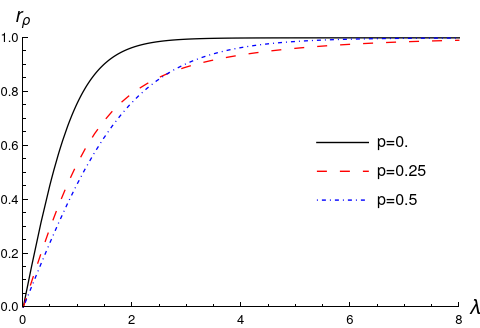
\includegraphics[width=0.8\columnwidth]{figures/r(lambda).png}%
                \caption{$r_{\rho}$ as a function of $\lambda$ for different values of $p$}
            \end{figure}
        \end{column}
    \end{columns}
\end{frame}
